\documentclass{scrreprt}
\usepackage{listings}
\usepackage{underscore}
\usepackage{graphicx}
\usepackage{wrapfig}
\usepackage{blindtext}
\usepackage[bookmarks=true]{hyperref}
\usepackage[utf8]{inputenc}
\usepackage[english]{babel}
\hypersetup{
	bookmarks=false,    % show bookmarks bar?
	pdftitle={Software Requirement Specification},    % title
	pdfauthor={Luis Mardueño},                     % author
	pdfsubject={TeX and LaTeX},                        % subject of the document
	pdfkeywords={TeX, LaTeX, graphics, images}, % list of keywords
	colorlinks=true,       % false: boxed links; true: colored links
	linkcolor=blue,       % color of internal links
	citecolor=black,       % color of links to bibliography
	filecolor=black,        % color of file links
	urlcolor=purple,        % color of external links
	linktoc=page            % only page is linked
}%
\def\myversion{2.0 }
\date{}
%\title
\usepackage{hyperref}
\begin{document}
	\begin{figure}
		
\includegraphics[width=50pt,height=50pt]{tecnm.PNG}
	\end{figure}
	
	\raggedright \large National Technological Institute of Mexico\vskip0.5cm
		\rule{20cm}{5pt}\vskip0.5cm
		\begin{bfseries}
			
			\begin{flushright}
			\Huge{SOFTWARE REQUIREMENTS\\ SPECIFICATION}\\
			\vspace{1.2cm}
			for\\
			\vspace{0.5cm}
			\Huge Web App for\\Medical Clinic\\
			\vspace{1.6cm}
			\LARGE Version \myversion approved\\
			\vspace{1.3cm}
			Prepared by author's\\
			\vspace{0.2cm}
			Jesus Lizárraga Rodriguez\\
			\vspace{0.2cm}
			Isabel Gutierrez Mora\\
			\vspace{0.2cm}
			Luis Mardueño Arroyo\\
			
			\vspace{0.7cm}
			\today\\
		\end{flushright}
		
		\end{bfseries}
	
		
	
	
	\tableofcontents
	
	
	\chapter{Introduction}
	
	\section{Purpose}
	The purpuse of this documents is to write down a set of problems that our client has and provide a web app solution. It is spected to have a sort of manual for the end users.
	
	\section{Document Conventions}
	This document uses the following conventions.
	\begin{itemize}
\item		DB 		Database
\item		DDB		Distributed Database
\item		ER 		Entity Relationship
\item		TCNM	National Technological Institute of Mexico
	\end{itemize}
	\section{Intended Audience and Reading Suggestions}
	This project is in a prototype stage for the development of our client page and it is restricted within our university. This has been implemented under the guidance of different TCNM. It is in our best interest for this paper to be approachable as possible to any reader regarding their background.
	
	
	\section{Project Scope}
	The scope of this project is to create a web solution to our client needs some of them are a way to store customer data, appointment management and
	given the costumer to know when their upcoming appointment.
	having a concise DB is critical for this project and all the benefits derive from having a easy way to interact with this data.
	
	
	
	\chapter{Overall Description}
	
	\section{Product Perspective}
	This client doesn't have a easy way to interact with their data everything is being done by hand and paper. Is up to the appointed person to keep track of any appointment to every client.
	
	The client lacks a web page where we must provide an interactive  way for costumers to check their appointments prescriptions, and attract new ones. to simplifly workflow for the administrive personel and phisicians 
	
	
	\section{Product Functions}
	
	The key features of the product are:
	\begin{itemize}
		\item	Data Storage and retrieval: Our web app provides a secure and scalable way to store, organize, and retrieve valuable client data. It is easy to use and ensures data integrity and accessibility.
		\item	User Authentication: Protect sensitive data with user validation controls. Grant and manage access privileges to ensure that only authorized users can view, edit, or manipulate specific data sets.
		\item Automated Reminders: Generate custom remainders notifications for patients appointments.
		\item Integration: Seamlessly integrate with the Web application and services.
	\end{itemize}
	
	
	\section{User Classes and Characteristics}
	We identify three user classes
	\begin{itemize}
		\item Patients should have to capability's of 
		\begin{itemize}
			\item Check their respective data
			\item Schedule new appointments
			\item Receive information about appointments and prescriptions
		\end{itemize}
		\item Doctors can perform different task like
		\begin{itemize}
			\item Schedule appointments
			\item Retrieve patient data
			\item Make a prescription 
		\end{itemize}
		\item Administrative personnel
		\begin{itemize}
			\item Register new users
			\item View specific parts of the patient clinical history
		\end{itemize}
	\end{itemize}
	
This are the major groups identified, but i could be integrated another classes thanks to our self hosting solution and ease of management

\pagebreak


	
	\section{ER Diagram}
	\subsection{Main tables:}
	Patients: This table will store general information about patients, such as their first name, last name, date of birth, social security number, address, etc.
	Physicians: This table will store information about physicians, such as their first name, last name, specialty, license number, etc.
	Appointments: this table will store information about appointments, such as date, time, duration, doctor, patient, etc.
	Hospitals : this table is to differentiate where the doctor is from and the address of the appointment.  
	Related tables:
	
	General Medical Records: This table will store general information about patients, such as their medical history, allergies, medications, etc.
	Specific medical records: this table will store specific information for each specialty, such as test results, prescriptions, etc.
	Relationships between tables:
	\begin{figure}[h]
		\centering
		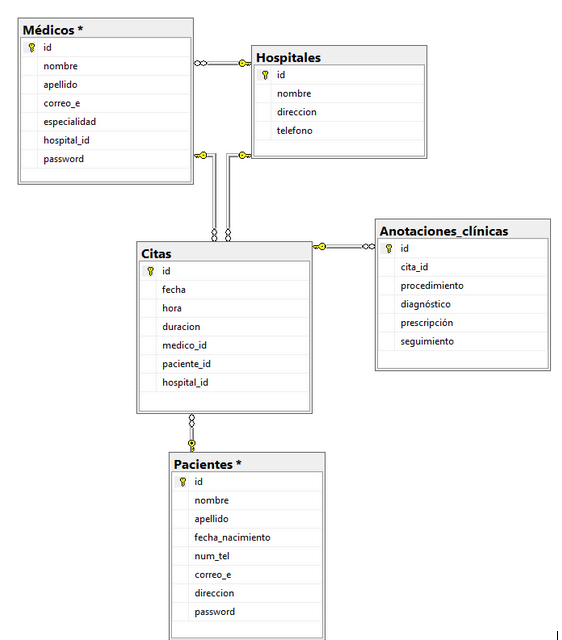
\includegraphics[width=300pt]{entidadrelacion.png}
		\caption{ER diagram}
		\label{fig:ER}
	\end{figure}
	
	\pagebreak
		\begin{figure}[h]
		\centering
		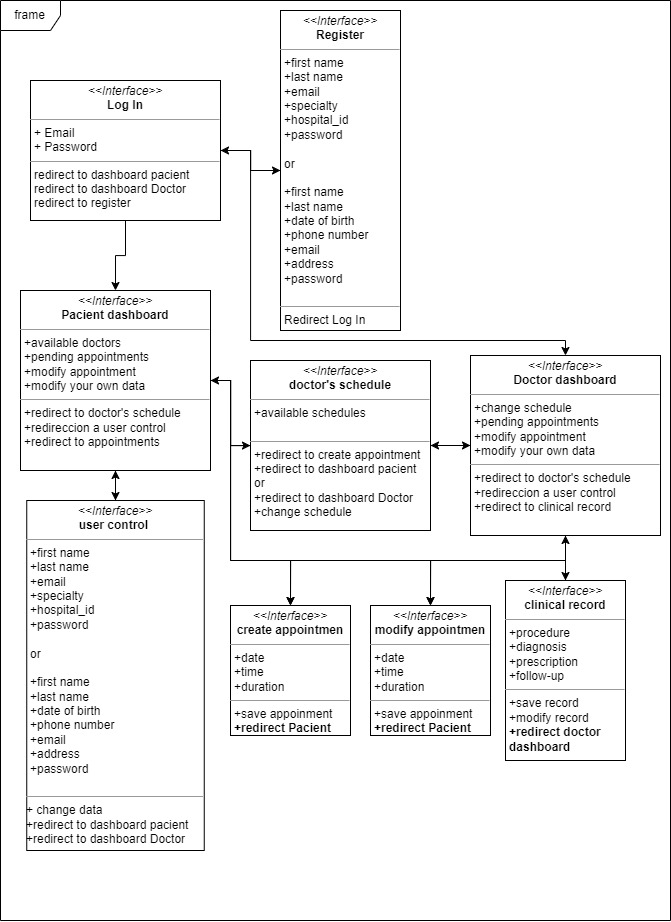
\includegraphics[width=300pt]{vistas.jpg}
		\caption{Views Diagrams}
		\label{fig:Diagram}
	\end{figure}
	\subsection{Patients:}
	 The Patients table has a one-to-many relationship with the General Medical Records table. This means that a patient can have several general medical records.
	Physicians: The Physicians table has a one-to-many relationship with the Appointments table. This means that a physician can attend several appointments.
	
	\subsection{Appointments:}
	 The Appointments table has a one-to-one relationship with the Specific Medical Records table. This means that an appointment can have only one specific medical record.
	Hospitals: will store appointment addresses and doctors. 
	
	
	\section{Operating Environment}
	The system for the ophthalmology clinic is designed to operate within a specific operating environment that must meet a range of technical and software requirements to ensure efficient and reliable operation. Below are detailed key components and considerations of the operating environment:
	\begin{itemize}
		\item Web server: The system utilizes a web server to provide access via a web browser. It can be deployed on common web servers such as Apache, Nginx, or other Python-compatible web servers like Flask or Django. The web server configuration should be appropriate to handle the expected traffic load, including multiple user requests, and ensure secure communication via HTTPS.
		
		\item Supported web Browsers: Users interact with the system through modern web browsers like Google Chrome, Mozilla Firefox, Microsoft Edge, and Safari. The web application should be compatible with these platforms and popular browsers. The use of standard web technologies and web standards is recommended to ensure compatibility.
		
	\end{itemize}
	
	
	\section{Design and Implementation Constraints}
	 Describe any items or issues that will limit the options available to the 
	developers. These might include: corporate or regulatory policies; hardware 
	limitations (timing requirements, memory requirements); interfaces to other 
	applications; specific technologies, tools, and databases to be used; parallel 
	operations; language requirements; communications protocols; security 
	considerations; design conventions or programming standards (for example, if the 
	customer’s organization will be responsible for maintaining the delivered 
	software).
	
	\section{User Documentation}
	 user documentation provides comprehensive guidance on using the appointment scheduling and clinical history management system for the ophthalmology clinic. It aims to help users, including medical professionals, staff, and administrators, make the most of the system's features and capabilities.
	 
	 Target Audience
	 This documentation is intended for all users of the system, including:
	 
	 Ophthalmologists
	 Clinic Staff (Assistants, Secretaries)
	 System Administrators
	 
	 For the patients they will require an easier guide to the activities that they can perform at the web page
	 \pagebreak
	\section{Assumptions and Dependencies}
	
	 In the development and implementation of the appointment scheduling and clinical history management system for the ophthalmology clinic, these are the important factors to consider as they can impact the project's scope, timeline, and successful execution.
	 
	 \begin{itemize}
	 \item	Clinic Infrastructure: It is assumed that the clinic already has the necessary hardware infrastructure, including servers or hosting services, network connectivity, and workstations, to support the system's operation.
	 	
	 \item	Internet Connectivity: Users are expected to have reliable internet access to use the system effectively. This includes both clinic staff and ophthalmologists who may access the system remotely.
	 	
	 \item	Data Accuracy: It is assumed that patient data provided to the system, such as personal information, medical history, and contact details, is accurate and up-to-date. Data inaccuracies can affect appointment scheduling and clinical record management.
	 	
	 \item	Compliance: The system is developed with the assumption that the clinic staff and users will adhere to all relevant legal and regulatory requirements, including data privacy laws such as HIPAA or GDPR, to ensure the confidentiality and security of patient information.
	 	
	 \item	User Training: Users are expected to receive adequate training and support to effectively use the system. Training materials and resources will be provided to assist users in becoming proficient with the system.
	 	
	 \end{itemize}
	
	
	\chapter{External Interface Requirements}
	
	\section{User Interfaces}
	User Interface Design Considerations:
	\begin{itemize}
\item User-Centered Design: Place the user at the center of your design process. Understand the needs and preferences of ophthalmologists, clinic staff, and other users to create interfaces that cater to their workflows and tasks.
	 
\item	 Consistency: Maintain a consistent look and feel throughout the application. Consistency in design elements, such as buttons, fonts, and colors, helps users navigate the system intuitively.
	 
\item	 Accessibility: Ensure that your interfaces are accessible to all users, including those with disabilities. Follow WCAG (Web Content Accessibility Guidelines) for accessibility standards.
	 
\item	 Responsive Design: Design interfaces that are responsive to different screen sizes and devices, including desktop computers, tablets, and smartphones.
	 
\item	 Information Hierarchy: Organize information logically, using clear hierarchies, headings, and grouping to help users find what they need quickly.
	 
\item	 Feedback and Confirmation: Provide feedback to users when actions are taken (e.g., successful appointment creation) and seek confirmation for critical actions (e.g., deleting a patient record).
	 
\item	 Efficiency: Streamline repetitive tasks and offer shortcuts to help users perform their duties efficiently. Consider keyboard shortcuts and quick actions.
	 
\item	 Error Handling: Clearly communicate errors to users with informative error messages. Suggest solutions or corrective actions when possible.
	\end{itemize}
	 
	
	\section{Hardware Interfaces}
	The appointment scheduling and clinical history management system for the ophthalmology clinic interacts with various hardware components and devices to support its functionality. This section describes the hardware interfaces and dependencies required for the system's operation.
	\section{Server Hardware}
	Description: The system operates on one or more servers machines that host the application and store data. 
	
	After rolling the first prototype into production we plan to use a single server
	
	
	\section{Software Interfaces}
	The appointment scheduling and clinical history management system for the ophthalmology clinic interacts with various software systems and components to support its functionality. This section describes the software interfaces and dependencies required for the system's operation.
	
	
	\section{Communications Interfaces}
	The appointment scheduling and clinical history management system for the ophthalmology clinic relies on various communication interfaces to facilitate data exchange, notifications, and interactions with external entities. This section describes the communication interfaces and protocols used by the system.
	\paragraph{User-System Communication}
	Description: User-System Communication refers to how users interact with the system's user interfaces through web browsers or client applications.
	
	Protocols and Interfaces:
	
	HTTP/HTTPS: User interactions with the system are primarily conducted via web browsers.
	
	
	
	\chapter{System Features}
	\section{Functional Requirements}
	
	\begin{itemize}
		\item Usability:
		The user interface must be intuitive and easy to use for clinic staff, even those with little technical experience.
		\item Performance:
		The system must be able to handle a significant number of appointments and clinical records without performance degradation.
		\item Security:
		Patient data must be protected through proper authentication and authorization. Medical information must be kept confidential.
		\item Scalability:
		The system must be able to adapt as the clinic grows, allowing for the addition of more physicians, patients and appointments.
		\item Availability:
		The system must be available during clinic operating hours so that staff can access it at any time.
		\item Data Backup:
		A data backup strategy should be implemented to ensure recovery in the event of data loss.
		
	\end{itemize}
	\section{Use Cases}
	Use cases are different uses where an actor can interact with the system.
	\pagebreak
	\subsection{Flow for Creating Patients}
	Use Case Flow for Creating Patients
	Actor: Clinic Staff
	Preconditions:\\
	
	Clinic staff must be authenticated in the system.
	Main Flow:\\
	
	Clinic staff enters patient information such as first name, last name, date of birth, address, and phone number.
	The system validates the patient's information.
	The system creates the patient in the database.
	The system displays a confirmation message.\\
	
	Extensions:\\
	
	If the patient information is incorrect, the system displays an error message.
	
	\begin{figure}[h]
		\begin{center}
			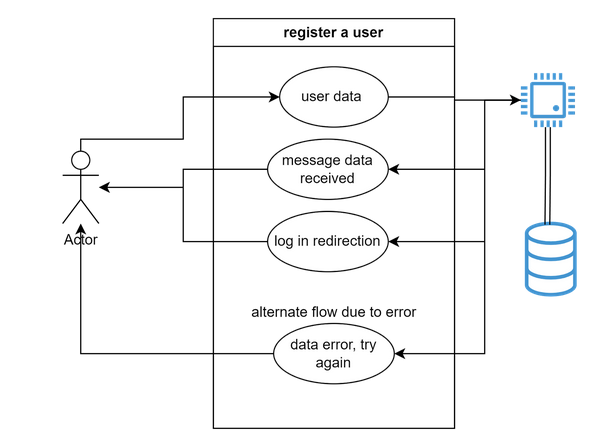
\includegraphics[width=350pt,height=180pt]{usuario1.png}
		\end{center}
		\label{fig:Use case 1}
	\end{figure}
	\pagebreak
	\subsubsection{Flow for Logging In}
	The doctor  must have an account registered in the system.
	Main Flow:\\
	
	The  user enters their username and password.
	The system validates the login information.
	The system authenticates user .
	The system displays the user interface corresponding to the user´s role.\\
	Extensions:\\
	
	If the login information is incorrect, the system displays an error message.It will also give the option to register 
	\begin{figure}[h]
		\begin{center}
			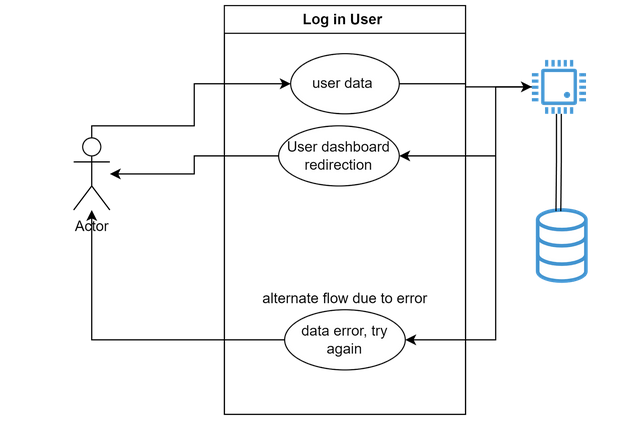
\includegraphics[width=350pt,height=280pt]{usuario2.png}
		\end{center}
		\label{fig:Use case 2}
	\end{figure}
	\pagebreak
	\subsubsection{Schedule an Appointment}
	Actor: Clinic Staff\\
	
	Main Flow:
	Staff requests schedule availability. 
	System responds to schedule availability 
	Clinic staff enters patient information, appointment date and time, and assigned medic
	The system confirms the appointment and assigns it to the patient.
	\begin{figure}[h]
		\begin{center}
			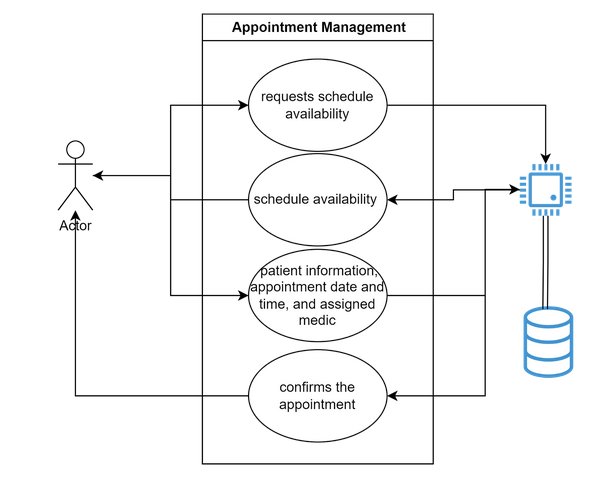
\includegraphics[width=350pt,height=280pt]{usuario3.png}
		\end{center}
		\label{fig:Use case 3}
	\end{figure}
	\pagebreak
	\subsubsection{Appointment Management}
	Use Case: Revise schedule
	Actor: Clinic Staff
	Precondition: User has the role of doctor. 
	Main Flow:
	User requests the schedule
	system responds with patient information, appointment dates and times
	User confirms appointment 
	system responds with saved information message
	
	\begin{figure}[h]
		\begin{center}
			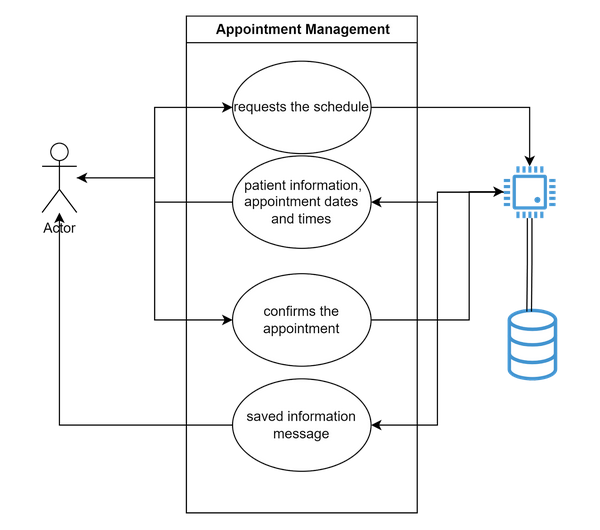
\includegraphics[width=350pt,height=280pt]{usuario4.png}
		\end{center}
		\label{fig:Use case 4}
	\end{figure}
	\pagebreak
	\subsubsection{ modify or delete appointment}
	Actor: patient or doctor
	precondition: user has the role of patient or doctor\\
	Main Flow:
	The user requests the schedule of his appointments 
	The system responds with the appointment dates and times.
	User modifies or deletes the appointment 
	system responds with saved information message
	\begin{figure}[h]
		\begin{center}
			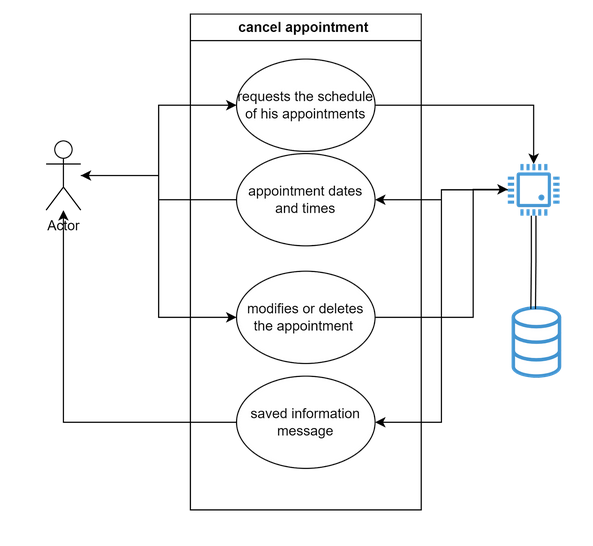
\includegraphics[width=350pt,height=280pt]{usuario5.png}
		\end{center}
		\label{fig:Use case 5}
	\end{figure}
	\pagebreak
	\subsubsection{ create clinical annotation }
	Actor: doctor
	precondition: user has the role of doctor\\
	Main Flow:
	The user requests the schedule of his appointments 
	The system responds with the appointment dates and times.
	User selects an appointment 
	user adds clinical annotations 
	system responds with saved information message
	\begin{figure}[h]
		\begin{center}
			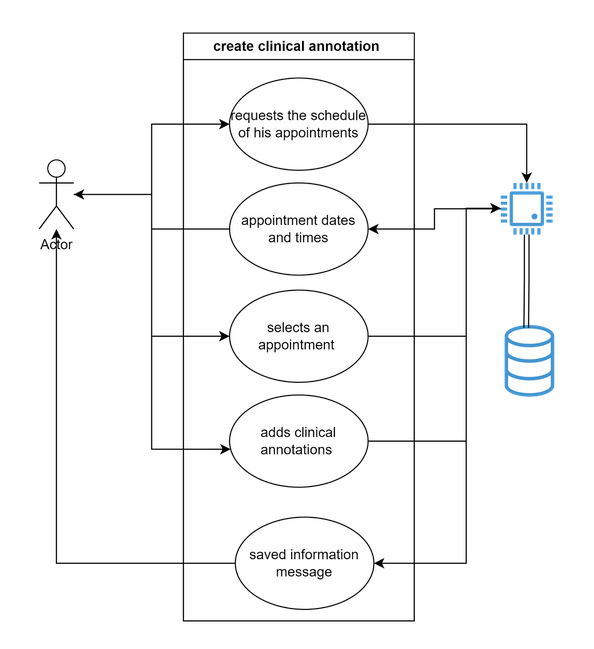
\includegraphics[width=350pt,height=280pt]{usuario6.png}
		\end{center}
		\label{fig:Use case 6}
	\end{figure}
	\pagebreak
	

	
	\subsubsection{Appointment Management}
	\begin{itemize}
	\item The system must allow clinic staff to schedule new appointments for patients, specifying the patient, date and time of the appointment.
	\item	It must be possible to modify or delete existing appointments.
	\item	The system should display appointment availability and avoid scheduling appointments at overlapping times.
	\end{itemize}
	 
	 
	
	\subsection{Description and Priority}
	The system needs a way to organize appointments and be checked by different users to ensure this we require the database to store information and the Web app to access it.\\
	This is the top priority of the system. The client states that has lost many data entries and had to be individual call for clarification meaning a crucial waste of resources. 
	
	\subsection{Stimulus/Response Sequences}
	 Patient comes or calls to the clinic makes a registry in the web app and is scheduled an appointment with their doctor witch checks the patient clinical history, makes a prescription and is giving the option to schedule another appointment for the next visit.
	
	
	
	\chapter{Other Nonfunctional Requirements}
	\section{Usability}
	The user interface must be intuitive and easy to use for clinic staff, even those with little technical experience.
	\section{Performance}
	The system must be able to handle a significant number of appointments and clinical records without performance degradation.
	\section{Scalability}
	The system must be able to adapt as the clinic grows, allowing for the addition of more physicians, patients and appointments.
	\section{Data backup}
	A data backup strategy should be implemented to ensure recovery in the event of data loss.
	
	
	
	
\end{document}